\documentclass{standalone}
\usepackage{tikz}
\usetikzlibrary{patterns, positioning}


\begin{document}
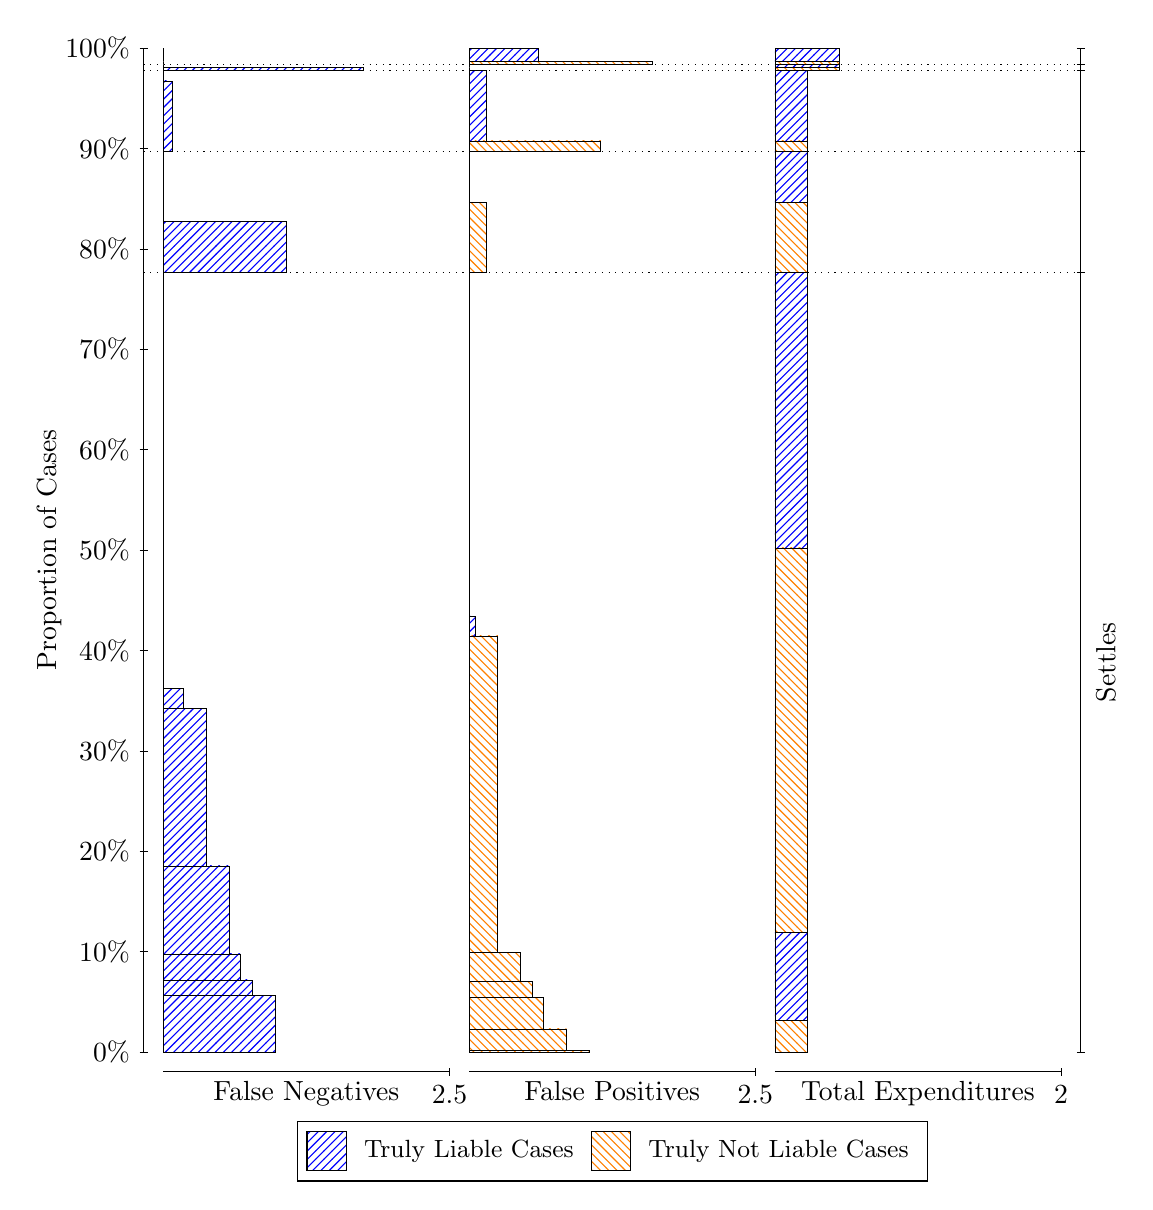
\begin{tikzpicture}
\draw[black, very thin] (1.5,1.75) -- (1.5,14.5);
\node[rotate=90, text=black, anchor=center] at (0.3, 8.125) {Proportion of Cases};
\draw[black, very thin] (1.45,1.75) -- (1.55,1.75);
\node[text=black, anchor=east] at (1.45, 1.75) {0\%};
\draw[black, very thin] (1.45,3.025) -- (1.55,3.025);
\node[text=black, anchor=east] at (1.45, 3.025) {10\%};
\draw[black, very thin] (1.45,4.3) -- (1.55,4.3);
\node[text=black, anchor=east] at (1.45, 4.3) {20\%};
\draw[black, very thin] (1.45,5.575) -- (1.55,5.575);
\node[text=black, anchor=east] at (1.45, 5.575) {30\%};
\draw[black, very thin] (1.45,6.85) -- (1.55,6.85);
\node[text=black, anchor=east] at (1.45, 6.85) {40\%};
\draw[black, very thin] (1.45,8.125) -- (1.55,8.125);
\node[text=black, anchor=east] at (1.45, 8.125) {50\%};
\draw[black, very thin] (1.45,9.4) -- (1.55,9.4);
\node[text=black, anchor=east] at (1.45, 9.4) {60\%};
\draw[black, very thin] (1.45,10.675) -- (1.55,10.675);
\node[text=black, anchor=east] at (1.45, 10.675) {70\%};
\draw[black, very thin] (1.45,11.95) -- (1.55,11.95);
\node[text=black, anchor=east] at (1.45, 11.95) {80\%};
\draw[black, very thin] (1.45,13.225) -- (1.55,13.225);
\node[text=black, anchor=east] at (1.45, 13.225) {90\%};
\draw[black, very thin] (1.45,14.5) -- (1.55,14.5);
\node[text=black, anchor=east] at (1.45, 14.5) {100\%};

\draw[black, very thin] (13.4,1.75) -- (13.4,14.5);
\draw[black, very thin] (13.35,1.75) -- (13.45,1.75);
\node[anchor=west] at (13.35, 1.75) {};
\draw[black, very thin] (13.35,11.65) -- (13.45,11.65);
\node[anchor=west] at (13.35, 11.65) {};
\draw[black, very thin] (13.35,13.187) -- (13.45,13.187);
\node[anchor=west] at (13.35, 13.187) {};
\draw[black, very thin] (13.35,14.217) -- (13.45,14.217);
\node[anchor=west] at (13.35, 14.217) {};
\draw[black, very thin] (13.35,14.288) -- (13.45,14.288);
\node[anchor=west] at (13.35, 14.288) {};
\draw[black, very thin] (13.35,14.5) -- (13.45,14.5);
\node[anchor=west] at (13.35, 14.5) {};

\draw[black, very thin, pattern color=blue, pattern=north east lines] (1.75,1.75) rectangle (3.167,2.4706);
\draw[black, very thin, pattern color=blue, pattern=north east lines] (1.75,2.4706) rectangle (2.8763,2.6663);
\draw[black, very thin, pattern color=blue, pattern=north east lines] (1.75,2.6663) rectangle (2.731,2.9969);
\draw[black, very thin, pattern color=blue, pattern=north east lines] (1.75,2.9969) rectangle (2.5857,4.1146);
\draw[black, very thin, pattern color=blue, pattern=north east lines] (1.75,4.1146) rectangle (2.295,6.1113);
\draw[black, very thin, pattern color=blue, pattern=north east lines] (1.75,6.1113) rectangle (2.0043,6.3656);
\draw[black, very thin, pattern color=orange, pattern=north west lines] (1.75,6.3656) rectangle (1.75,11.65);
\draw[black, very thin, pattern color=blue, pattern=north east lines] (1.75,11.65) rectangle (3.3123,12.302);
\draw[black, very thin, pattern color=orange, pattern=north west lines] (1.75,12.302) rectangle (1.75,13.187);
\draw[black, very thin, pattern color=blue, pattern=north east lines] (1.75,13.187) rectangle (1.859,14.084);
\draw[black, very thin, pattern color=orange, pattern=north west lines] (1.75,14.084) rectangle (1.75,14.217);
\draw[black, very thin, pattern color=blue, pattern=north east lines] (1.75,14.217) rectangle (4.2933,14.256);
\draw[black, very thin, pattern color=orange, pattern=north west lines] (1.75,14.256) rectangle (1.75,14.288);
\draw[black, very thin, pattern color=orange, pattern=north west lines] (1.75,14.288) rectangle (1.75,14.328);
\draw[black, very thin, pattern color=blue, pattern=north east lines] (1.75,14.328) rectangle (1.75,14.5);
\draw[black, very thin, pattern color=orange, pattern=north west lines] (5.6333,1.75) rectangle (7.1593,1.7682);
\draw[black, very thin, pattern color=orange, pattern=north west lines] (5.6333,1.7682) rectangle (6.8687,2.0431);
\draw[black, very thin, pattern color=orange, pattern=north west lines] (5.6333,2.0431) rectangle (6.578,2.448);
\draw[black, very thin, pattern color=orange, pattern=north west lines] (5.6333,2.448) rectangle (6.4327,2.6416);
\draw[black, very thin, pattern color=orange, pattern=north west lines] (5.6333,2.6416) rectangle (6.2873,3.0165);
\draw[black, very thin, pattern color=orange, pattern=north west lines] (5.6333,3.0165) rectangle (5.9967,7.0346);
\draw[black, very thin, pattern color=blue, pattern=north east lines] (5.6333,7.0346) rectangle (5.706,7.2889);
\draw[black, very thin, pattern color=blue, pattern=north east lines] (5.6333,7.2889) rectangle (5.6333,11.65);
\draw[black, very thin, pattern color=orange, pattern=north west lines] (5.6333,11.65) rectangle (5.8513,12.535);
\draw[black, very thin, pattern color=blue, pattern=north east lines] (5.6333,12.535) rectangle (5.6333,13.187);
\draw[black, very thin, pattern color=orange, pattern=north west lines] (5.6333,13.187) rectangle (7.3047,13.32);
\draw[black, very thin, pattern color=blue, pattern=north east lines] (5.6333,13.32) rectangle (5.8513,14.217);
\draw[black, very thin, pattern color=orange, pattern=north west lines] (5.6333,14.217) rectangle (5.6333,14.25);
\draw[black, very thin, pattern color=blue, pattern=north east lines] (5.6333,14.25) rectangle (5.6333,14.288);
\draw[black, very thin, pattern color=orange, pattern=north west lines] (5.6333,14.288) rectangle (7.9587,14.328);
\draw[black, very thin, pattern color=blue, pattern=north east lines] (5.6333,14.328) rectangle (6.5053,14.5);
\draw[black, very thin, pattern color=orange, pattern=north west lines] (9.5167,1.75) rectangle (9.9254,2.1549);
\draw[black, very thin, pattern color=blue, pattern=north east lines] (9.5167,2.1549) rectangle (9.9254,3.2726);
\draw[black, very thin, pattern color=orange, pattern=north west lines] (9.5167,3.2726) rectangle (9.9254,8.1522);
\draw[black, very thin, pattern color=blue, pattern=north east lines] (9.5167,8.1522) rectangle (9.9254,11.65);
\draw[black, very thin, pattern color=orange, pattern=north west lines] (9.5167,11.65) rectangle (9.9254,12.535);
\draw[black, very thin, pattern color=blue, pattern=north east lines] (9.5167,12.535) rectangle (9.9254,13.187);
\draw[black, very thin, pattern color=orange, pattern=north west lines] (9.5167,13.187) rectangle (9.9254,13.32);
\draw[black, very thin, pattern color=blue, pattern=north east lines] (9.5167,13.32) rectangle (9.9254,14.217);
\draw[black, very thin, pattern color=orange, pattern=north west lines] (9.5167,14.217) rectangle (10.334,14.25);
\draw[black, very thin, pattern color=blue, pattern=north east lines] (9.5167,14.25) rectangle (10.334,14.288);
\draw[black, very thin, pattern color=orange, pattern=north west lines] (9.5167,14.288) rectangle (10.334,14.328);
\draw[black, very thin, pattern color=blue, pattern=north east lines] (9.5167,14.328) rectangle (10.334,14.5);
\draw[black, dotted] (1.5,11.65) -- (13.4,11.65);
\draw[black, dotted] (1.5,13.187) -- (13.4,13.187);
\draw[black, dotted] (1.5,14.217) -- (13.4,14.217);
\draw[black, dotted] (1.5,14.288) -- (13.4,14.288);
\draw[black, very thin] (1.75,1.5) -- (5.3833,1.5);
\node[text=black, anchor=north] at (3.5667, 1.5) {False Negatives};
\draw[black, very thin] (5.3833,1.45) -- (5.3833,1.55);
\node[text=black, anchor=north] at (5.3833, 1.45) {2.5};

\draw[black, very thin] (5.6333,1.5) -- (9.2667,1.5);
\node[text=black, anchor=north] at (7.45, 1.5) {False Positives};
\draw[black, very thin] (9.2667,1.45) -- (9.2667,1.55);
\node[text=black, anchor=north] at (9.2667, 1.45) {2.5};

\draw[black, very thin] (9.5167,1.5) -- (13.15,1.5);
\node[text=black, anchor=north] at (11.333, 1.5) {Total Expenditures};
\draw[black, very thin] (13.15,1.45) -- (13.15,1.55);
\node[text=black, anchor=north] at (13.15, 1.45) {2};

\node[text=black, centered, rotate=90] at (13.72, 6.7001) {Settles};





\draw (7.449999999999999,1.5) node[draw=none] (baseCoordinate) {};
\begin{scope}[align=center]
        \matrix[scale=0.5, draw=black, below=0.5cm of baseCoordinate, nodes={draw}, column sep=0.1cm]{
            \node[rectangle, draw, minimum width=0.5cm, minimum height=0.5cm, pattern color=blue, pattern=north east lines] {}; &
            \node[draw=none, font=\small, text=black] (B) {Truly Liable Cases}; &
            \node[rectangle, draw, minimum width=0.5cm, minimum height=0.5cm, pattern color=orange, pattern=north west lines] {}; &
            \node[draw=none, font=\small, text=black] (B) {Truly Not Liable Cases}; \\
            };
\end{scope}

\end{tikzpicture}
\end{document}